\section{Hardware}

\begin{frame}{Equipamento: Lemonbot}
    
    \begin{minipage}{0.6\textwidth}
        \begin{itemize}
            \item Plataforma portátil e autónoma capaz de realizar aquisições.
            \item Tem 3 partes funcionais:
            \begin{itemize}
                \item Laser Lidar
                \item Câmara RGB
                \item Pan-Tilt Unit (PTU)
            \end{itemize}
        \end{itemize}
    \end{minipage}%
    \begin{minipage}{0.4\textwidth}
        \begin{tikzpicture}
            \tikzset{
                frame/.style={rectangle, draw=black},
                link/.style={thick}
            }
            \node[frame] (ptu) {PTU};
            \node[frame, below=of ptu] (base) {Base};
            \node[frame, above left=of ptu, xshift=0.05cm] (laser) {Laser};
            \node[frame, above right=of laser, xshift=0.05cm] (camera) {Câmara};
                                                
            \draw[link] (base.north) -| (ptu.south);
            \draw[link] (ptu.west) -| (laser.south);
            \draw[link] (laser.east) -| (camera.south);            
        \end{tikzpicture}
    \end{minipage}

\end{frame}

\begin{frame}{Laser}

    \begin{minipage}{0.6\textwidth}
        
        Laser Lidar Sick LMS100

        \begin{itemize}
            \item 2D ou planar
            \item Radiação Infra-vermelhos
            \item Resolução de 12mm
            \item Abertura de 270º
            \item Intervalo 0.5m .. 30m
        \end{itemize}

    \end{minipage}%
    \begin{minipage}{0.4\textwidth}
        \begin{figure}
            \centering
            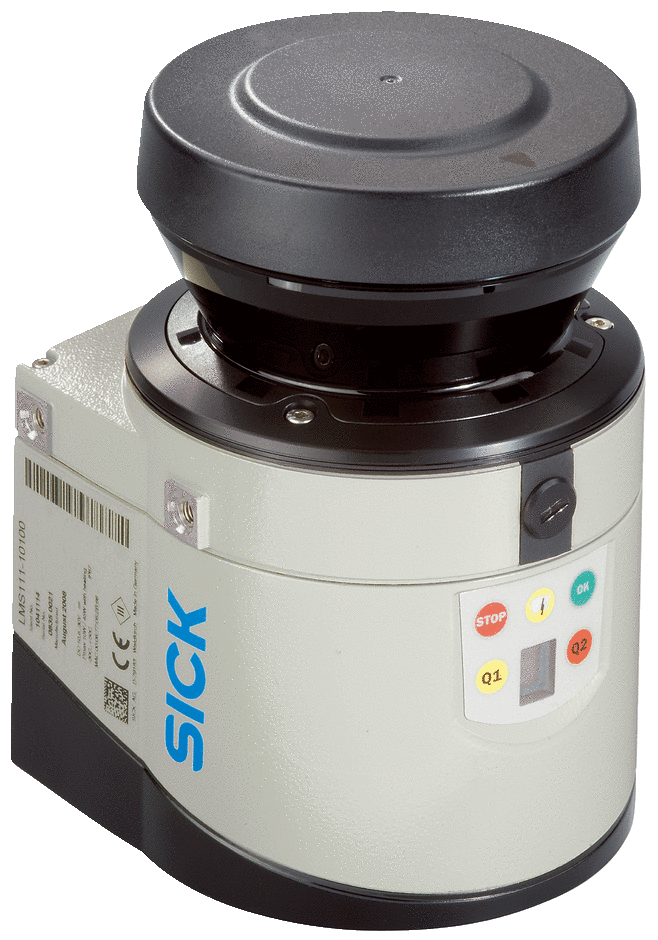
\includegraphics[width=0.8\textwidth]{img/laser.png}
        \end{figure}
    \end{minipage}
    
\end{frame}

\begin{frame}{Câmara}
    
    \begin{minipage}{0.6\textwidth}
        
        Câmara PointGrey Flea3

        \begin{itemize}
            \item 2.8 MP
            \item Resolução 1920x1440px
            \item Framerate 15 fps
        \end{itemize}

    \end{minipage}%
    \begin{minipage}{0.4\textwidth}
        \begin{figure}
            \centering
            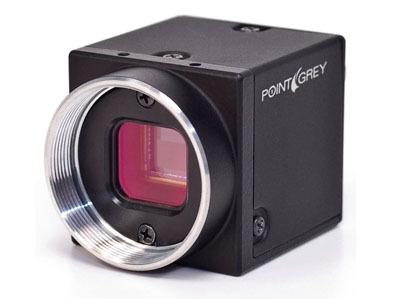
\includegraphics[width=0.8\textwidth]{img/flea3.jpg}
        \end{figure}
    \end{minipage}

\end{frame}

\begin{frame}{PTU}
    
    \begin{minipage}{0.6\textwidth}
        
        FLIR Pan-Tilt D46

        \begin{itemize}
            \item Tilt -45º..+45º
            \item Pan -146º..+146º
            \item Precisão Elevada 0.01º
        \end{itemize}

    \end{minipage}%
    \begin{minipage}{0.4\textwidth}
        \begin{figure}
            \centering
            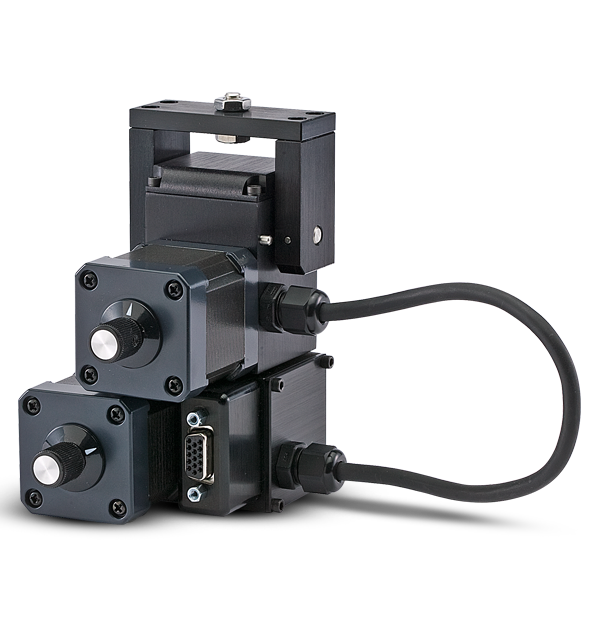
\includegraphics[width=1\textwidth]{img/ptu-d46.png}
        \end{figure}
    \end{minipage}

\end{frame}